%%%%%%%%%%%%%%%%
\chapter{Methodology}
\label{methods}
    %%%%%%%%%%%%%%%%
    \section{Instruments}
    %% Add efficiency of both detectors with respect to wavelength to explain why we choose 5000 rather that 4000 in general and in particular for BG Cru when looking at the second periodicity(why it's bigger).
        \begin{figure}[H]
        \centering
        \begin{subfigure}{.45\textwidth}
            \centering
            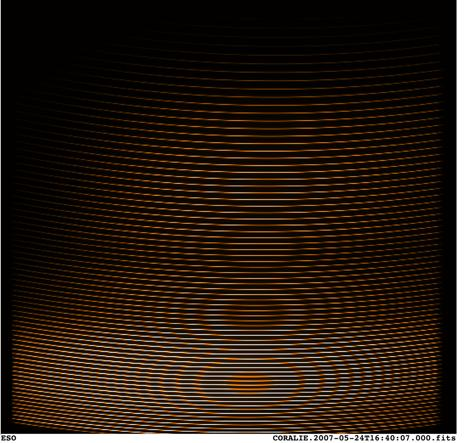
\includegraphics[width=0.8\textwidth]{report/images/chap3_methods/coralie_grating.jpg}
            \vspace{2em}
        \end{subfigure}%
        \hspace{1em}
        \begin{subfigure}{.45\textwidth}
            \centering
            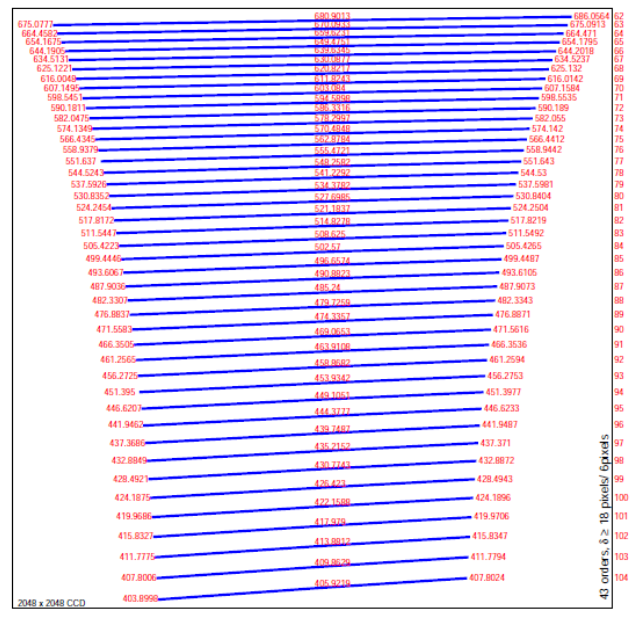
\includegraphics[width=\textwidth]{report/images/chap3_methods/echellogram.png}
        \end{subfigure}
        \caption{???}
        \label{3.1a}
        \end{figure}

        \begin{figure}[H]
        \centering
        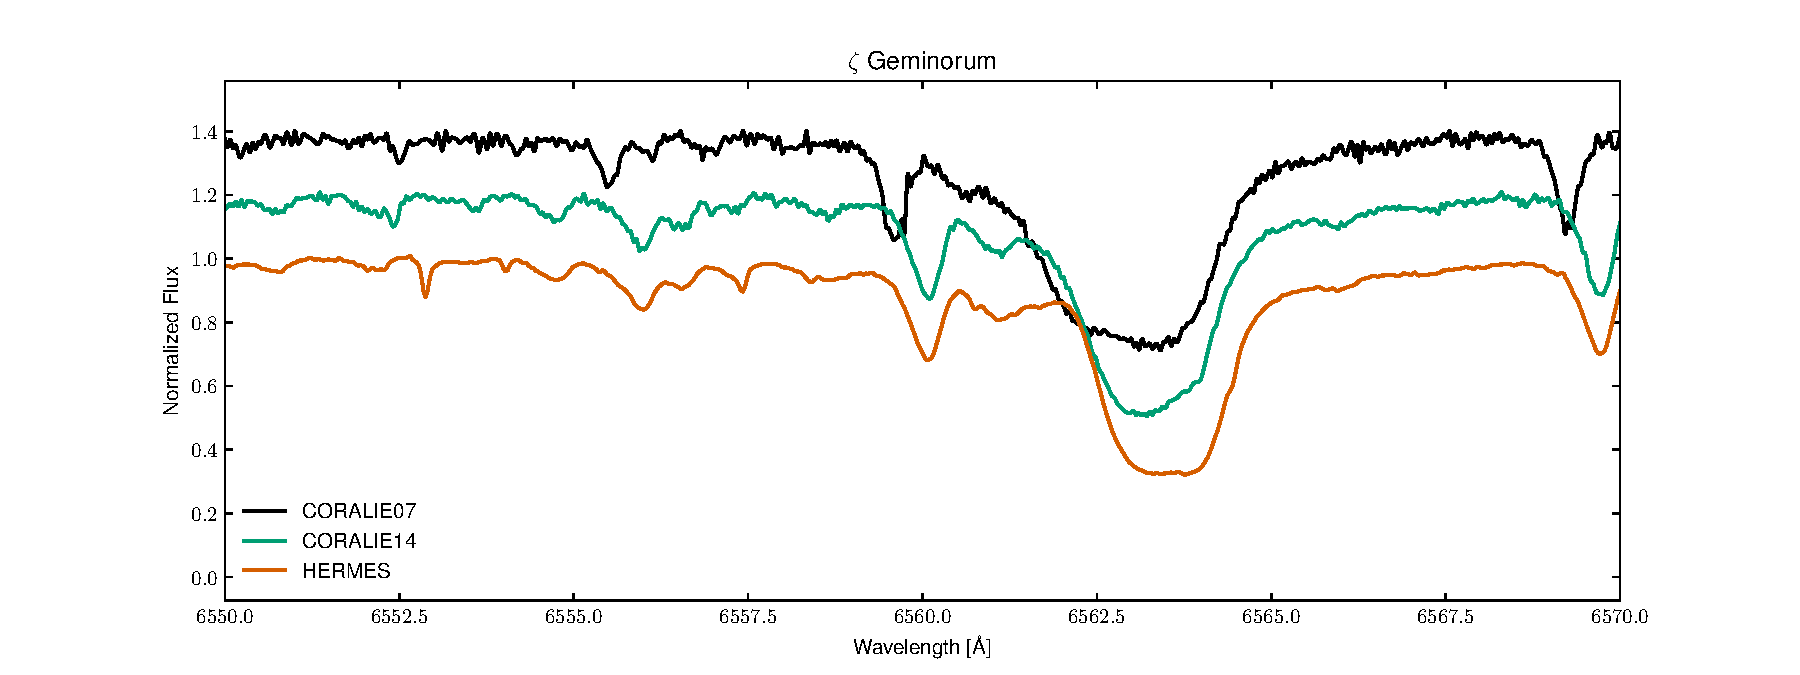
\includegraphics[width=\textwidth]{report/images/chap3_methods/zetgem_hermes_coralie.pdf}
        \caption{Caption}
        \label{3.1b}
        \end{figure}
    
        \subsection{CORALIE}
            \subsubsection{CORALIE07}
            \subsubsection{CORALIE14}
        \subsection{HERMES}
        \begin{figure}[H]
        \centering
        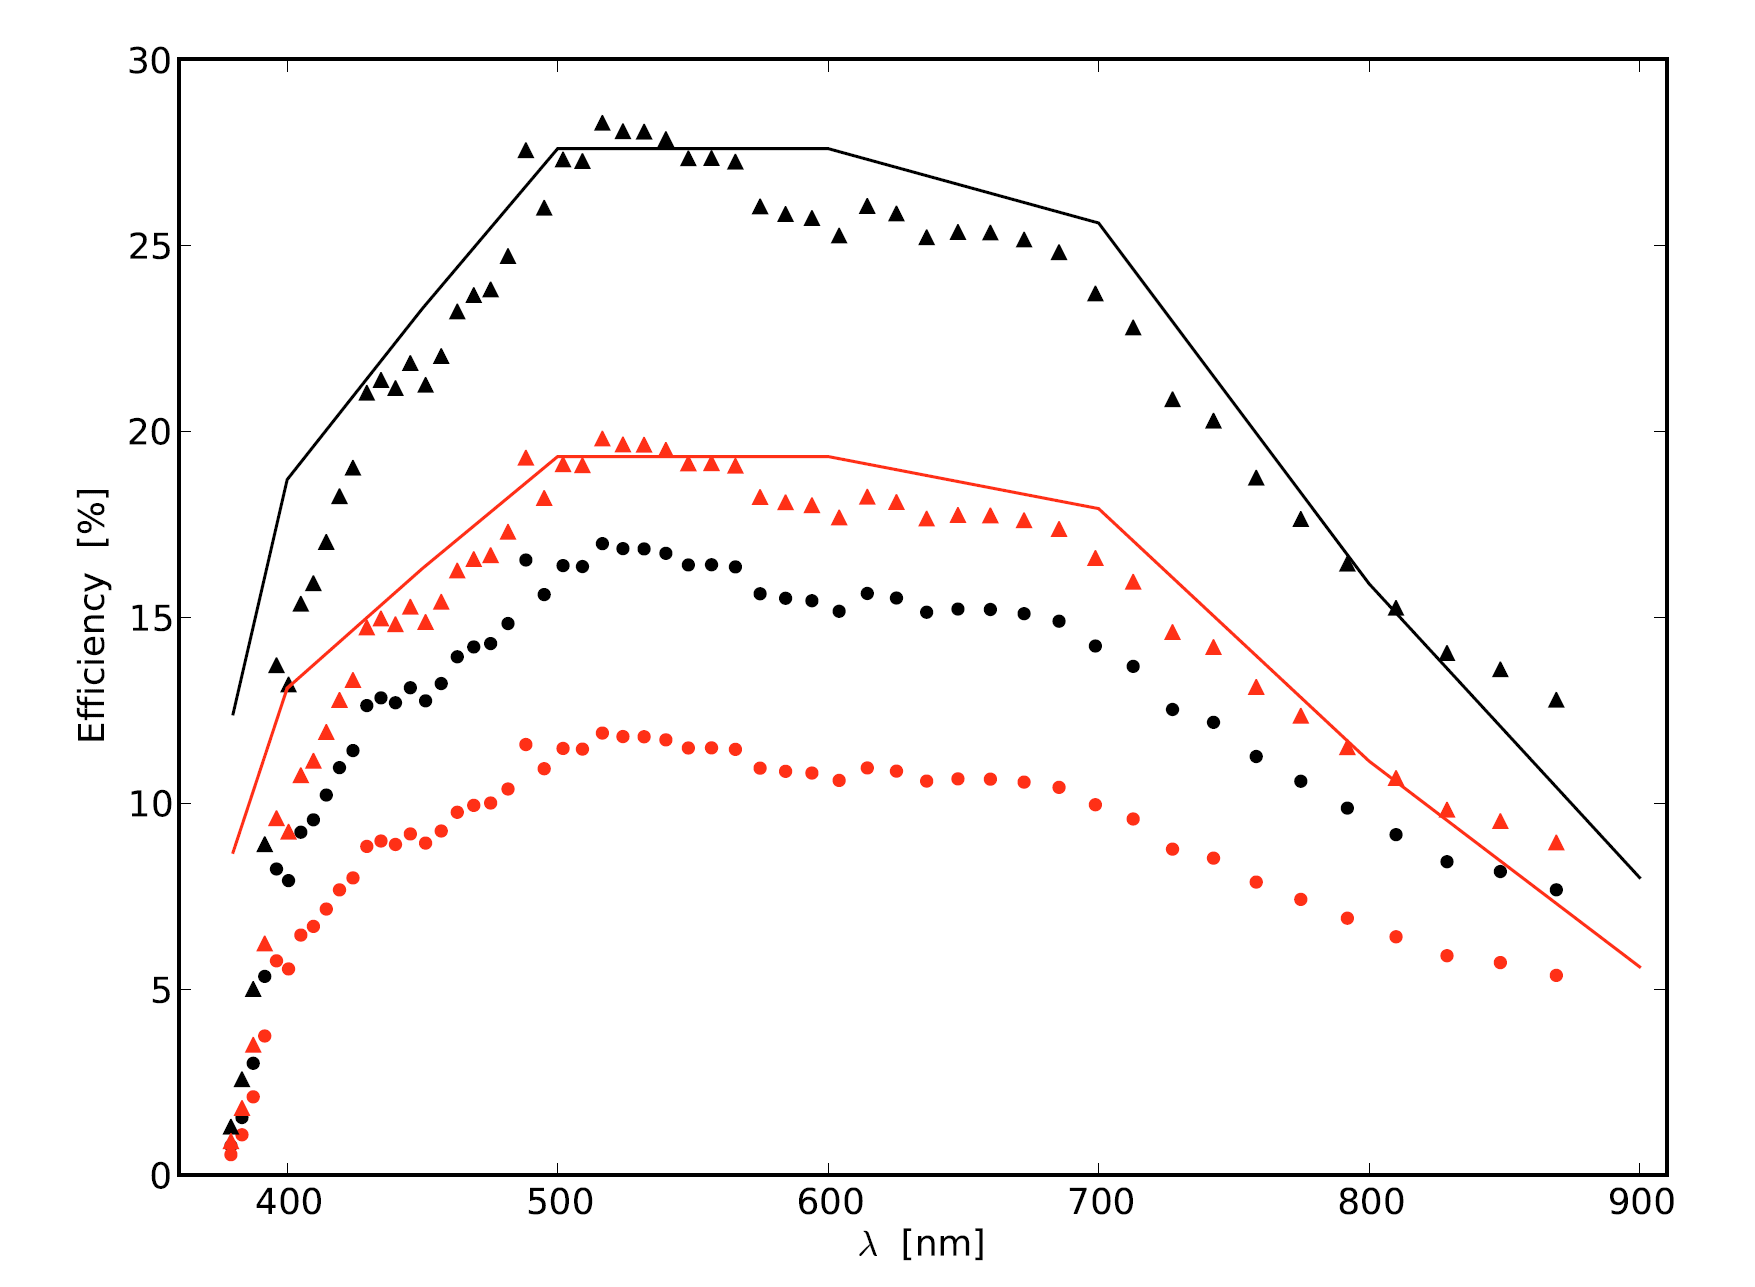
\includegraphics[width=0.6\textwidth]{report/images/chap3_methods/efficiency_hermes.png}
        \caption{Caption}
        \label{3.1c}
        \end{figure}
    \section{Data}
    %say data post and after 2018 for hermes + coralie7 and 14
    \subsection{Spectra}
    \subsection{Radial Velocities}
    \section{The SPARTA package}
    %Explain how it works step by step
    \subsection{Spectrum preprocessing}

        \begin{figure}[H]
        \centering
        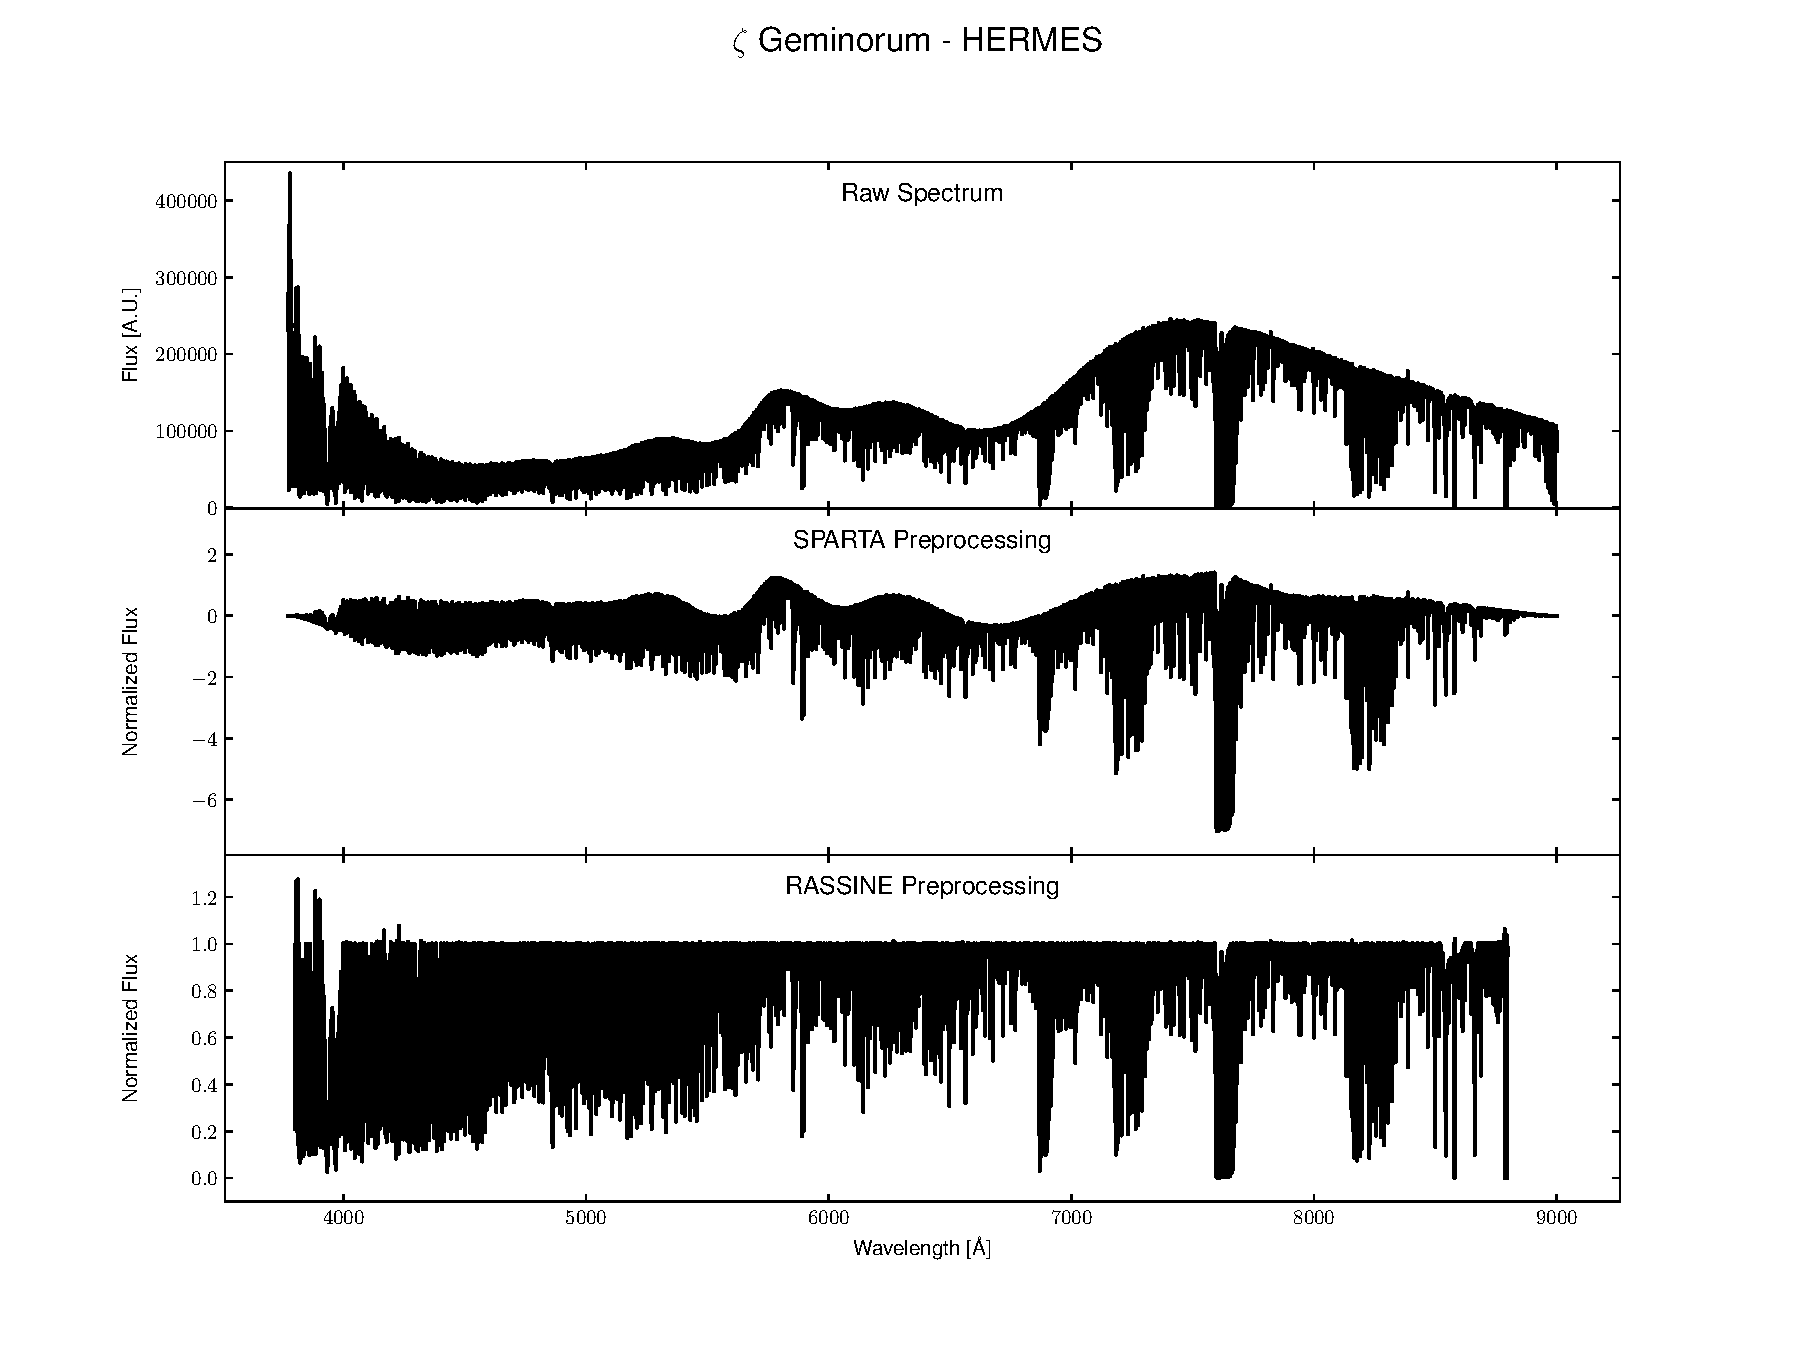
\includegraphics[width=\textwidth]{report/images/chap3_methods/zetgem_preprocessing_hermes.pdf}
        \caption{Caption}
        \label{3.3a}
        \end{figure}

        \begin{figure}[H]
        \centering
        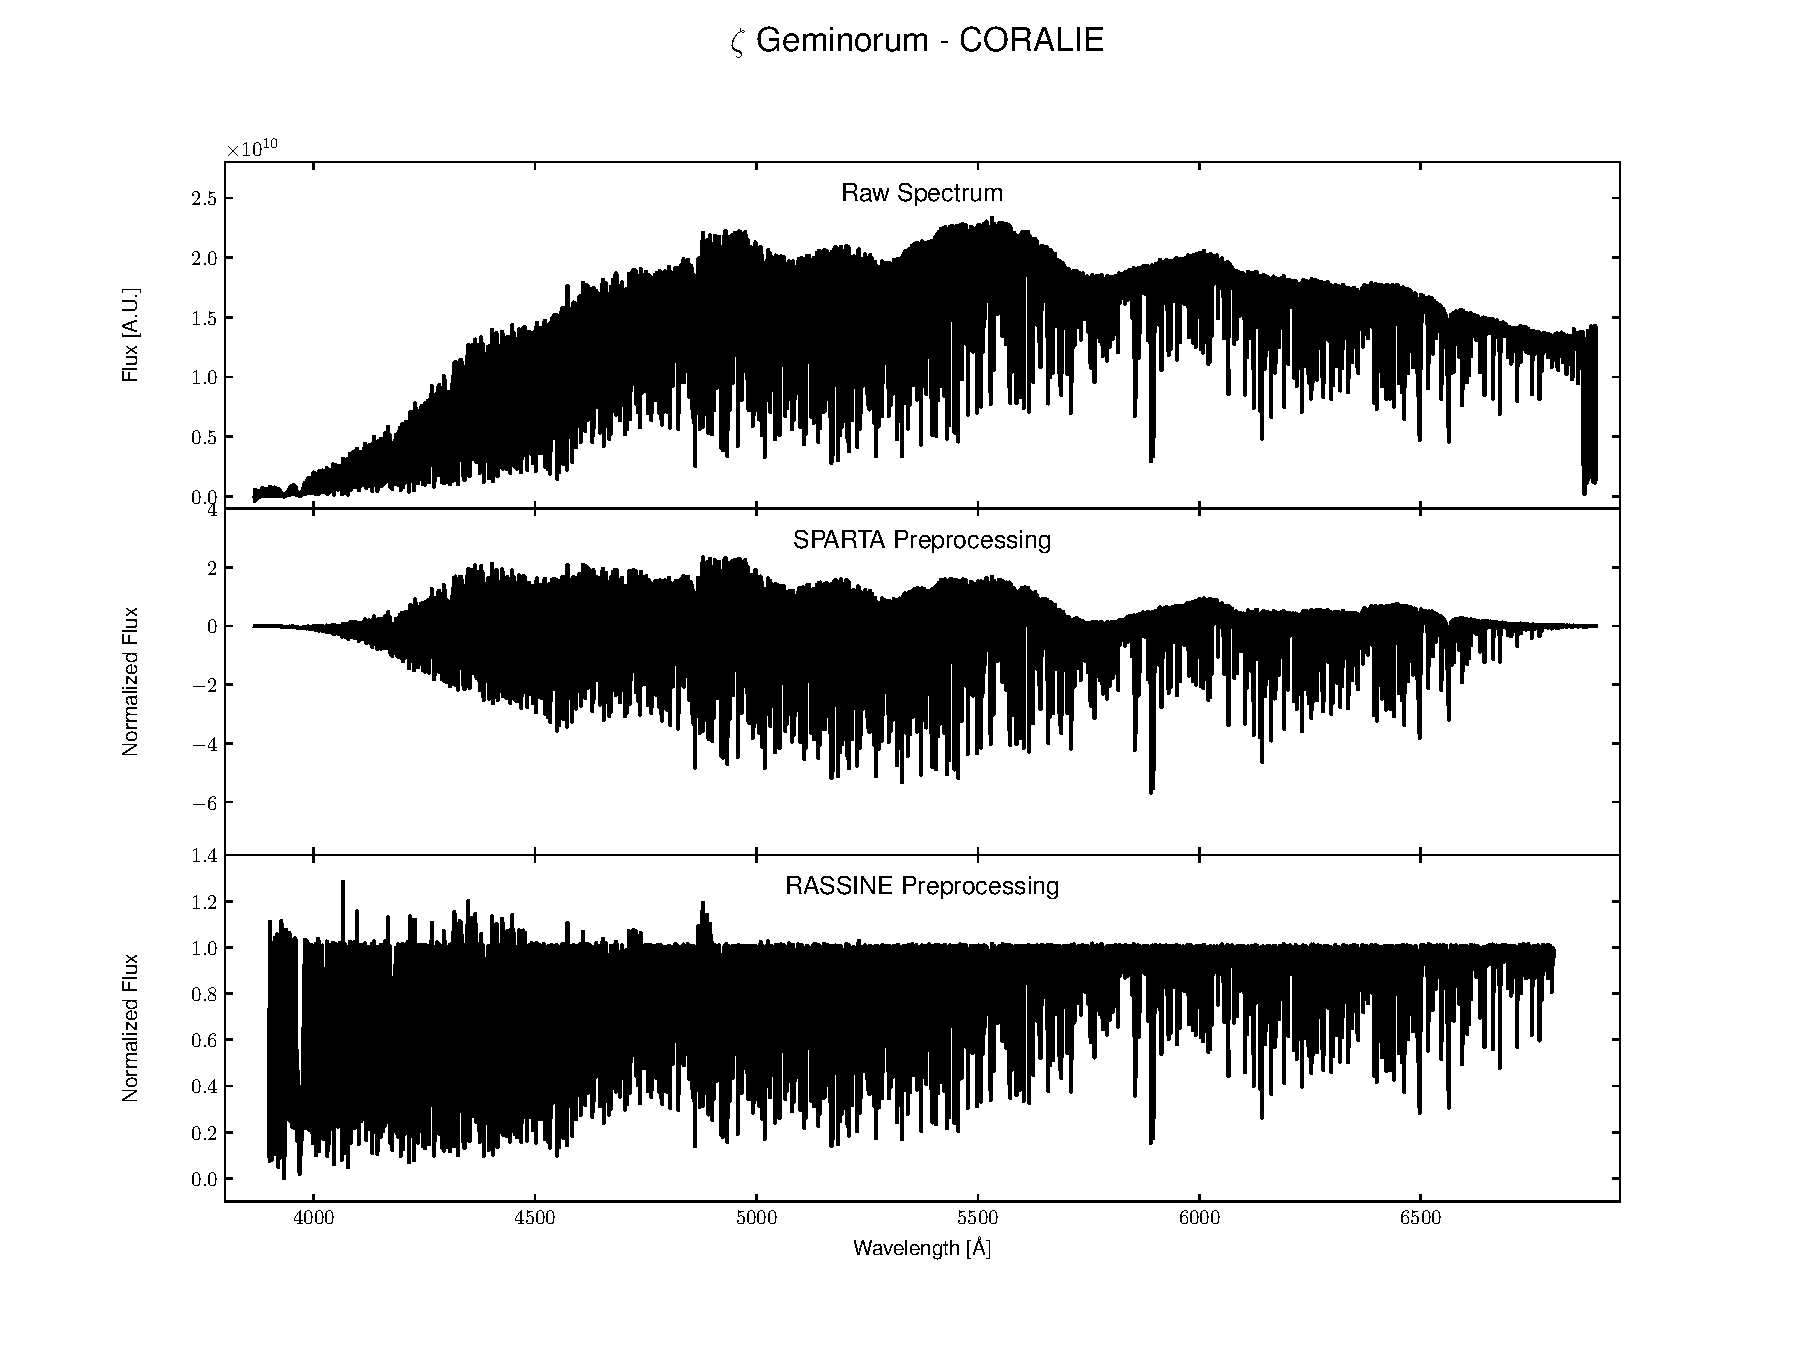
\includegraphics[width=\textwidth]{report/images/chap3_methods/zetgem_preprocessing_coralie14.pdf}
        \caption{Caption}
        \label{3.3b}
        \end{figure}
    
    \subsubsection{The RASSINE method}
    %explain why you use continuum linear and not cubic
    \section{Asserting a peak's statistical significance}
    %explain that in gls and non uniformly sampled periodograms in general, the harmonics and aliases are less power than in uniformly sampled data.

        \begin{figure}[H]
        \centering
        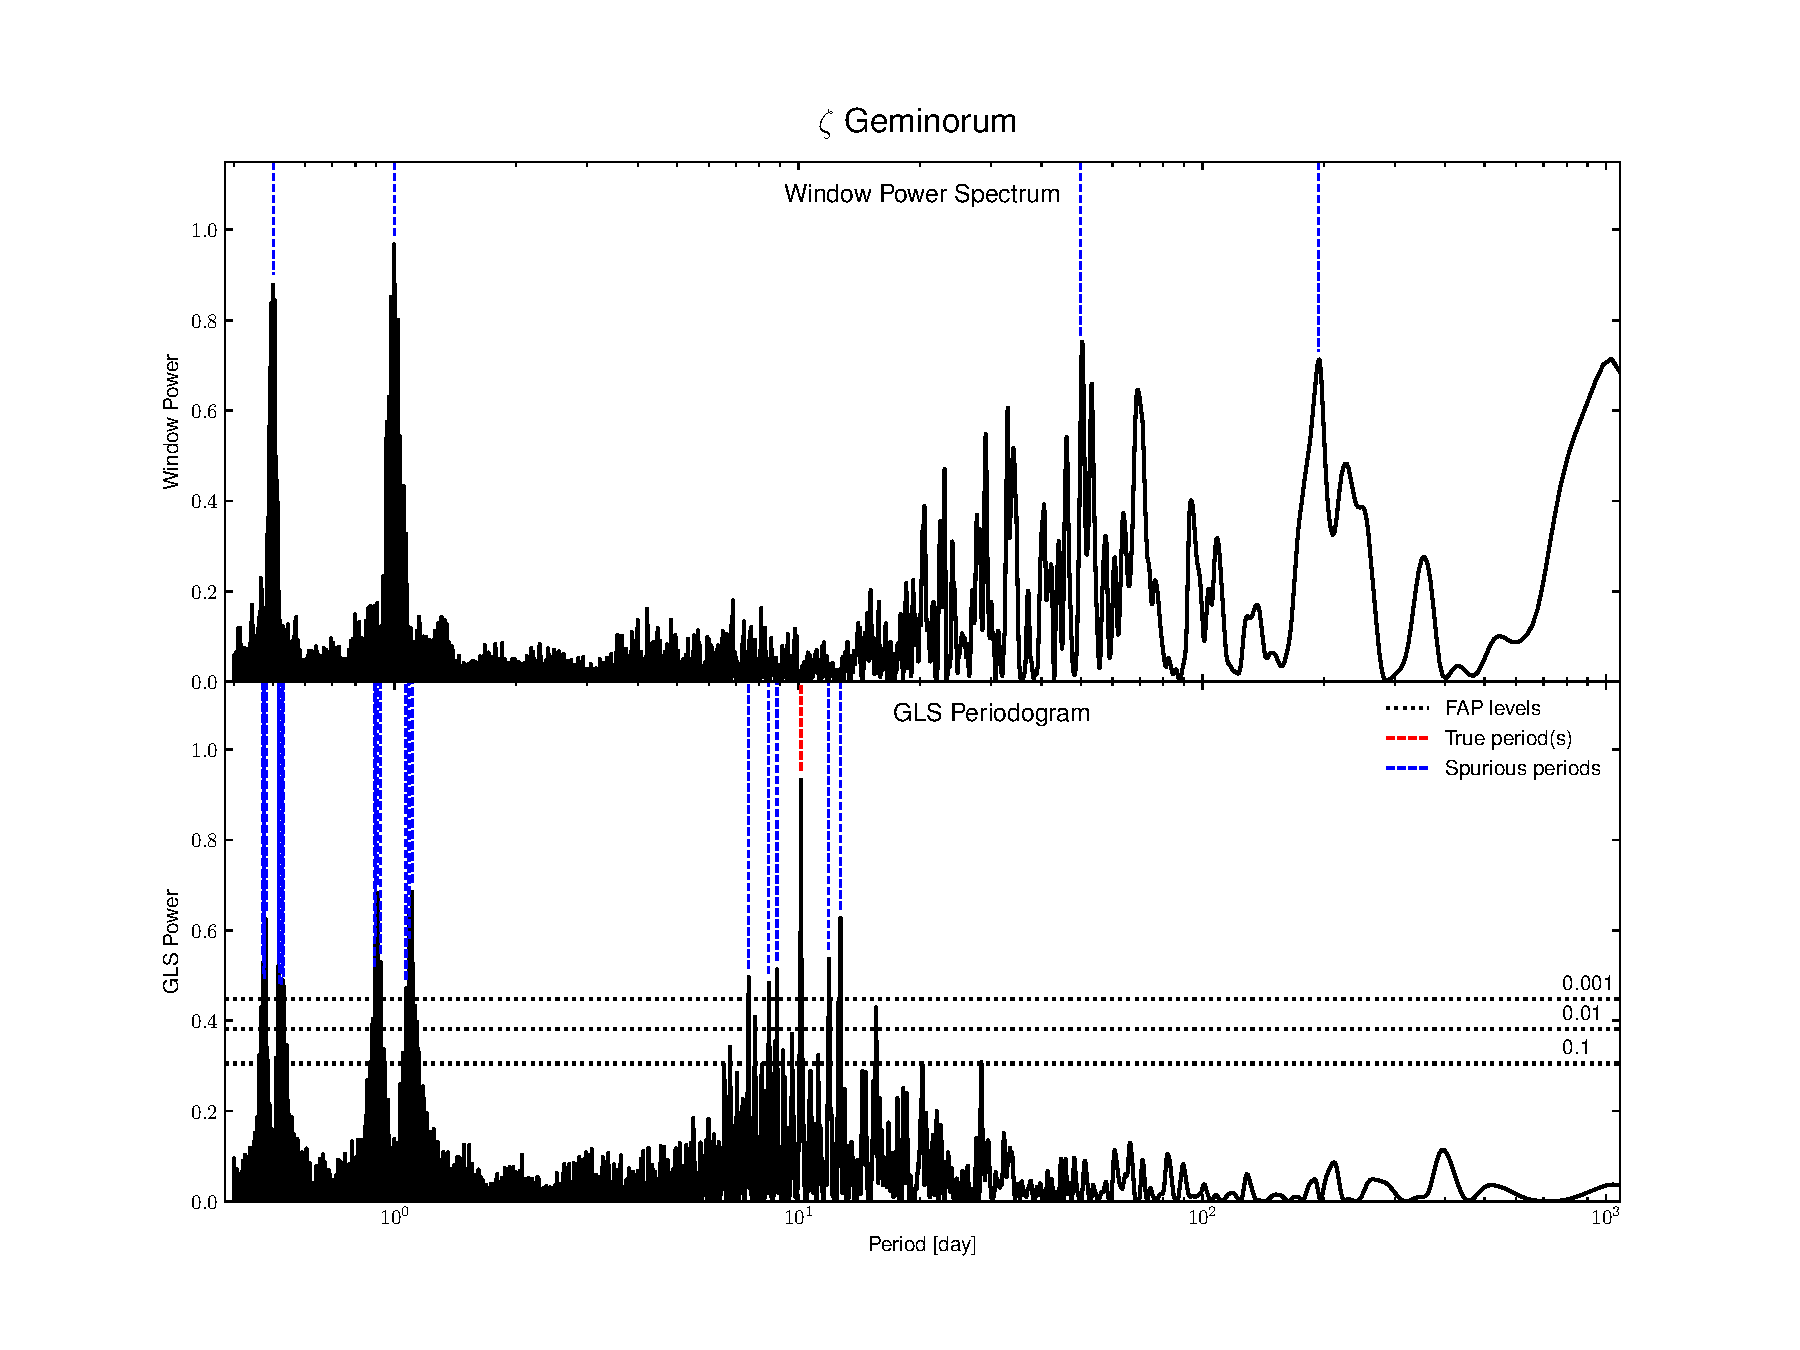
\includegraphics[width=\textwidth]{report/images/chap3_methods/windows_examples.pdf}
        \caption{Caption}
        \label{3.4a}
        \end{figure}
    \subsection{Window functions}
    \subsection{Failure modes: harmonics and aliases}
    \subsection{False-alarm rates and p-values}
as